The event selection aims to identify events with one or two leptons and a Lorentz-boosted $V$ boson produced with VBS topology. Candidate events with a tightly identified lepton with $\pt>30\GeV$ target the $\PW V \rightarrow \ell \nu V$ decays, characterized by a significant amount of missing transverse energy ($\ptmiss$) associated to the undetected neutrino. The Drell-Yan and QCD multi-jet background processes are reduced by requiring $\ptmiss>50\GeV$ ($\ptmiss>80\GeV$) in the muon (electron) final state. 

Candidate events with two same flavor leptons of opposite charges with  $\pt>30\GeV$ target the  $\PZ V \rightarrow \ell \ell V$ decays. The candidate $Z$ boson invariant mass is required to lie within $15\GeV$ of the nominal $\PZ$ boson mass.

Events are required to have at least one $V$-tagged jet with $\pt>200\GeV$, $\abs{\eta}<2.4$, and $65~\GeV < m_{V} < 105~\GeV$. In the case of multiple $V$ candidates, the one with mass closest to the nominal $\PW$ boson mass is selected.  The events are required to contain at least two jets with $\pt>30\GeV$ and $\abs{\eta}<5.0$, and $\Delta R(j,V)>0.8$. In the case of more than two jet candidates, the pair with the largest dijet mass is selected. The VBS topology is targeted by requiring a large dijet mass $m_{jj}>800\GeV$, and a large pseudorapidity separation $\abs{\Delta \eta_{jj}}>4.0$.  

Events with three or more loosely identified leptons with $\pt>20\GeV$ and $\abs{\eta}<2.5\,(2.4)$ for electrons (muons) are rejected. Identification of b-quark jets with $\pt$ greater than 30 $\GeV$ and lying within the tracker fiducial region ($\left|\eta\right|<2.4$)  is used to further reject top quark background events.   

The longitudinal component of the neutrino momentum in $\PW V \rightarrow \ell \nu V$ events is estimated by constraining the mass of the lepton and neutrino system to be the nominal $\PW$ boson mass~\cite{Sirunyan:2018iff}. The resulting quadratic equation is solved using $\vec{\mathrm{p}}_{T}^{\mathrm{miss}}$ as an estimate of the neutrino $\vec{\mathrm{p}}_{T}$.

Additional selection criteria are then used to enhance the sensitivity to AQGCs. Candidate events are required to have  $z_{V}^{*} < 0.3$ and $z_{W}^{*} < 0.3$, where $z_{V}^{*} = \abs{\eta_{V}-(\eta_{j1}+\eta_{j2})/2}/\abs{\Delta \eta_{jj}}$ is the Zeppenfeld variable~\cite{Rainwater:1996ud}, $\eta_{V}$ is the
pseudorapidity of a gauge boson, and $\eta_{j1}$ and $\eta_{j2}$ are the pseudorapidities of the leading and subleading jet, respectively. In addition, events are required to have $\vartheta>1.0$ where $\vartheta = \mathrm{min}(\mathrm{min}(\eta_{W},\eta_{V})-\mathrm{min}(\eta_{j1},\eta_{j2}),\mathrm{min}(\eta_{j1},\eta_{j2})-\mathrm{min}(\eta_{W},\eta_{V}))$ is the so called boson centrality. 

Statistical analysis of the event yields is performed with a fit to the mass distribution of the $\PW V$ or $\PZ V$ system. The mass distributions are binned as follows: $m_{\PW V}$ = [$600$,$1075$,$1550$,$2025$,$\infty$]. The distributions of $m_{\PW V}$ and $m_{\PZ V}$ in the signal region are shown in Figure~\ref{fig:signal2}. The data yield together with the SM expectation for the different processes is given in Table~\ref{tab:sel_yields15}.


\begin{figure*}[htb]
\centering
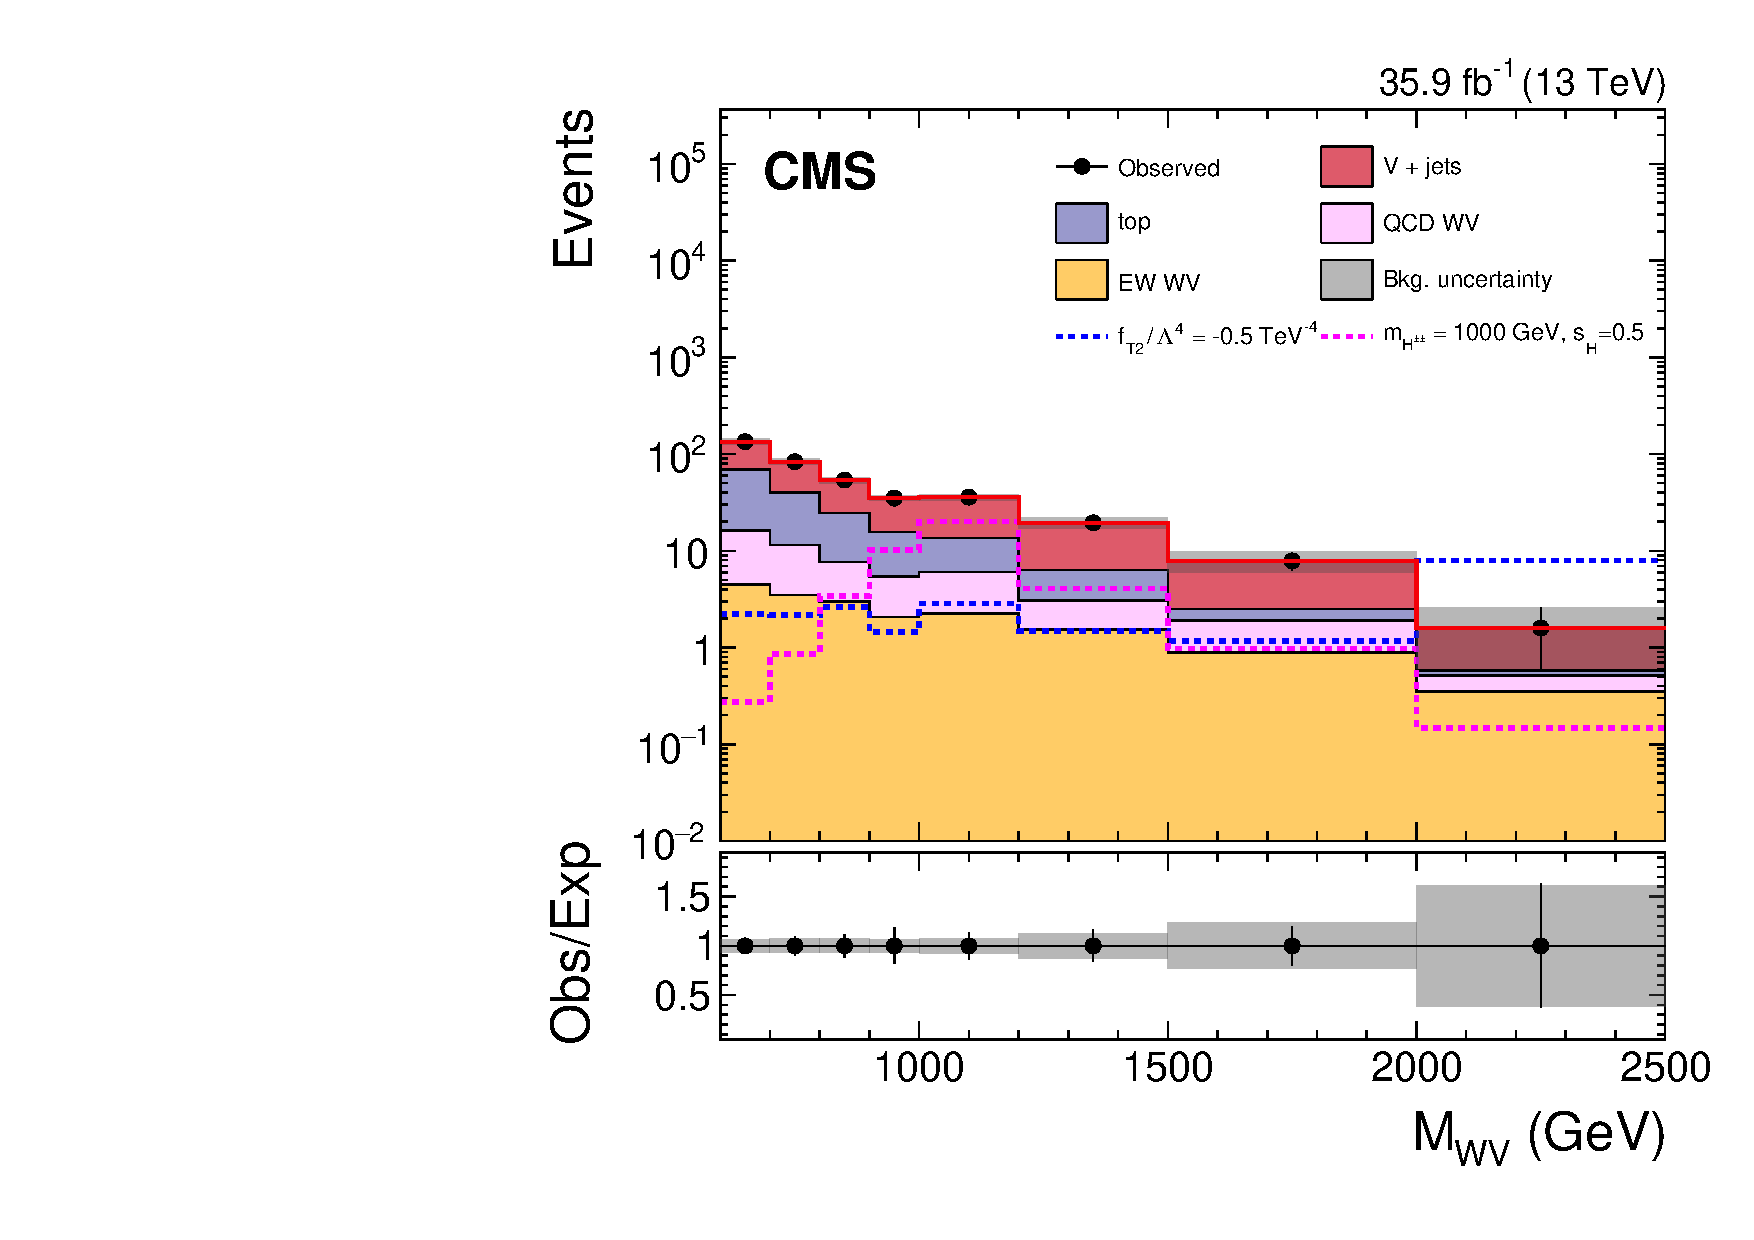
\includegraphics[width=\cmsFigWidth]{Plots/plots/wv_signal.pdf}
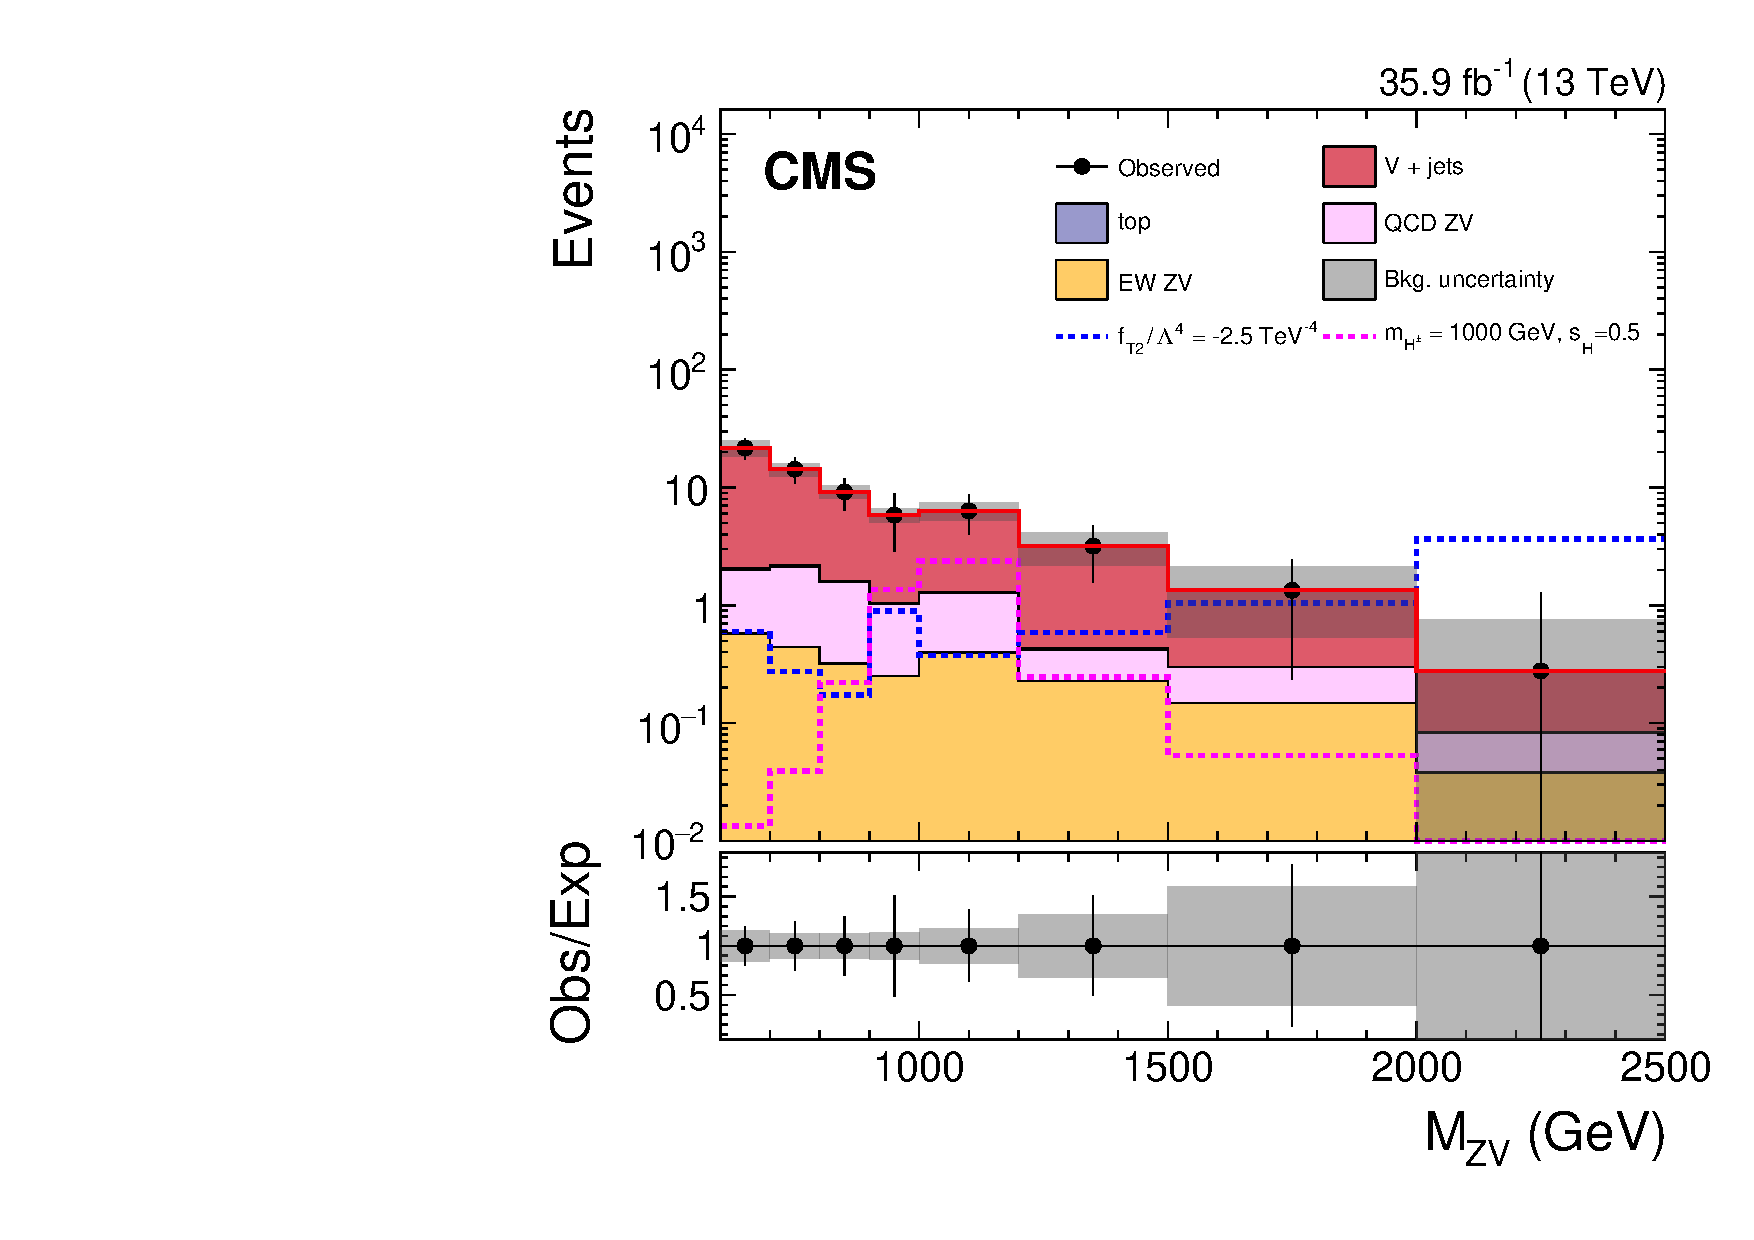
\includegraphics[width=\cmsFigWidth]{Plots/plots/zv_signal.pdf}
\caption{Distributions of $m_{WV}$ (left) and $m_{ZV}$ (right) in
the signal region. The hatched bands include statistical uncertainties from the predicted yields.The histograms for other backgrounds include the contributions
from QCD initiated dibosons, top, $\PW+$jets, and Drell--Yan processes. The overflow is included in the last bin.}
\label{fig:signal2}
\end{figure*}


\begin{table}[htbp]
\topcaption{Expected yields from various background processes in $\PW V$ and $\PZ V$ final states. Only the statistical uncertainties are shown. The SM EW signal yields are also shown.
\label{tab:sel_yields15}}
  \centering
  \newcolumntype{x}{D{,}{\,\pm\,}{3.3}}
  \begin{scotch}{lx{c}@{\hspace*{5pt}}x}
Final state   	      &   \multicolumn{1}{c}{$\PW V$} &&  \multicolumn{1}{c}{$\PZ V$}	       	    \\
\cline{2-2}\cline{4-4}
Data                  &   \multicolumn{1}{c}{\NA}   && \multicolumn{1}{c}{\NA}               \\
\hline
$\PW+$jet    	      &   223 ,  2  &&    0.0 ,  0.0    \\
$\PZ+$jet    	      &   2 ,  2  &&    48 ,  6     \\
top       	      &   136 ,  5  &&    0.1 ,  0.1   \\
QCD diboson  	      &   39 ,  1  &&    7 ,  1      \\
\hline
Total bkg.           &    410 ,  6   &&    55 ,  6   \\[1ex]
EW signal             &  24 , 2 && 2.5 , 0.1\\
\end{scotch}
\end{table}
